\documentclass[10pt,oneside,slovak,a4paper]{article}

\usepackage[slovak]{babel}
%\usepackage[T1]{fontenc}
\usepackage[IL2]{fontenc} % lepšia sadzba písmena Ľ než v T1
\usepackage[utf8]{inputenc}
\usepackage{graphicx}
\usepackage{url} % príkaz \url na formátovanie URL
\usepackage{hyperref} % odkazy v texte budú aktívne (pri niektorých triedach dokumentov spôsobuje posun textu)
\usepackage{booktabs}

\usepackage{cite}
%\usepackage{times}
\usepackage{indentfirst}
\pagestyle{headings}

\title{Kahoot! v E-learningu\thanks{Semestrálny projekt v predmete Metódy inžinierskej práce, ak. rok 2020/21, vedenie: Fedor Lehocki}} % meno a priezvisko vyučujúceho na cvičeniach

\author{Adam Škurla\\[2pt]
	{\small Slovenská technická univerzita v Bratislave}\\
	{\small Fakulta informatiky a informačných technológií}\\
	{\small \texttt{xskurla@stuba.sk}}
	}

\date{\small 15. október 2020}



\begin{document}

\maketitle

\begin{abstract}
V tejto práci sledujeme použitie Kahoot! v E-learningu ako súčasť game-based learningu. Kahoot! je vzdelávacia platforma založená na hre a interaktívnej forme kvízov, kde študenti môžu ihneď reagovať a zlepšuje to ich komunikáciu s učiteľom počas učiva. Kahoot! je aplikácia, ktorá sa momentálne používa najmä kvôli tomu, že študent dostane takmer okamžitú spätnú väzbu. V tejto práci , by sme sa chceli zaoberať s tým, ako študenti a aj učitelia zlepšili svoje výsledky práve pomocou aplikácie Kahoot!. Študentom sa zvýšila úspešnosť na vyučovacích predmetoch práve vďaka tejto aplikácii. Dôvodom je najmä to, že väčšina študentov si túto aplikáciu pochvaľovala najmä preto lebo mohli lepšie a rýchlejšie reagovať a učitelia mohli vytvárať omnoho lepšie otázky a dať tak študentom omnoho lepšie skúsenosti pri výučbe.
\end{abstract}



\section*{Úvod}
\label{uvod}
V posledných rokoch môžeme sledovať zvýšený nárast popularity používania mobilu alebo inej technológie ako súčasť výučby. Tento nárast umožnilo najmä to, že dnes  vlastní smartfón až 3,5 miliard ľudí, čo je 44,81\% svetovej populácie\cite{Turner2020} a toto číslo bude už len narastať. Technológie sa už dostali vo veľkom aj do škôl, kde uľahčujú prácu učiteľom a zároveň zlepšujú motiváciu študentov sa učiť. Najmä hry a interaktívne formy učenia si získali na škole veľké publikum. Študenti totižto viac obľubujú hravú formu učenia, vo forme súťaží, kvízov alebo hrania inej hry\cite{WANG2020}. Prebúdza to v nich väčšiu pozornosť a skôr sa tak sústredia a zapamätajú si nové učivo. Pre učiteľov je zase pozitívum to, že väčšinou tieto technológie a aplikácie nie sú ťažké a tak sa s nimi naučia rýchlo pracovať, zároveň tak dostávajú lepšiu spätnú väzbu od svojich študentov ako rozumejú učivu, lebo im súčasne môže odpovedať aj viac študentov naraz. Medzi také obľúbené herne aplikácie pri učení patria Socrative, Quizlet alebo Kahoot!.\cite{Licorish} Práve Kahoot! je z týchto aplikácii najslávnejší a najčastejšie používaní.  

	Cieľom tohto článku je predstaviť aplikáciu Kahoot!, ktorá sa v poslednej dobe dostala vo výučbe do popredia, uvedieme schopnosti a vlastnosti tejto aplikácie, ukážeme jej pozitíva a negatíva a v závere sa pozrieme aj na experiment, ktorý potom celý zhodnotíme. Ešte predtým ako si toto cele povieme si musíme vysvetliť, čo znamená pojem game-based learning.






\section{Game-based learning (Učenie založené na hraní hier)} \label{ml}

Game-based e-learning je v dnešnej dobe celkom normálny spôsob učenia na škole, napriek tomu aj tak nemá presnú definíciu. Za game-based learning môžeme považovať taký štýl učenia, kde použitie videohry podporuje výučbu učitela a zároveň pomáha žiakovi sa lepšie učiť.\cite{Perrota}
	
	Mnoho ľudí keď sa povie slovo videohra, tak si to predstavia ako aktivitu, ktorá nás len oberá o čas pri učení, preto si to poďme pozrieť z pohľadu učiteľa a študenta\cite{Perrota}. Z pohľadu študenta môže použitie videohry pri učení mať viacero možností, môže sa totižto naučiť niečo nové a zároveň zažiť srandu, brať to ako výzvu alebo ako súťaž a prekonávať svoje maximum v hre alebo súťažiť s kamarátom\cite{Perrota}. Veľa študentov uvádza, že práve hranie videohier ich naučilo cudzí jazyk. 
	
	Z pohľadu učiteľa je použitie videohry ako štýl učenia najmä kvôli tomu aby sa priblížil ku novej generácii študentov s médiom, ktoré poznajú aj oni. Učitelia môžu pri vysvetľovaní nejakej novej témy odporučiť svojim študentom hru, ktorá prehĺbi alebo dokonca zlepší ich vedomosti z daného učiva\cite{Perrota}. 
	
	Game-based learning sa dá použiť aj najmä na zlepšenie komunikácie medzi učiteľmi a študentmi. Učitelia použijú aplikácie ako slid.io alebo Kahoot!, kde napíšu napríklad nejakú otázku a študent cez mobil alebo iné zariadanie môže napísať alebo si vybrať správnu odpoveď. Zlepšuje to tak spätnú väzbu medzi učiteľmi a študentami, keďže sa do toho dokáže zapojiť omnoho vyššie množstvo študentov. U študentov zároveň stúpa ochota a motivácia splniť zadanie od učitelia, práve kvôli tomu, že to je cez videohru.\cite{Perrota} Študenti sa aj ochotnejšie zapájajú lebo väčšina video hier a aplikácii umožňuje aby sa študenti prihlasovali pod anonymným menom a nemusia sa báť výsmechu z prípadnej zlej odpovede.
	
	Stručne povedané, game-based learning je momentálny častý spôsob vyučovania na škole a to najmä kvôli, že študenti sa môžu cez svoje mobilné zariadenia aktívnejšie zapájať do výučby.



\section{Čo je aplikácia Kahoot!} \label{ina}
Kahoot! je online aplikácia, ktorá je na stiahnutie zadarmo a môže byť používaná pre všetkých učiteľov na rôznych úrovniach a pre rôzne predmety[3]. Táto aplikácia obsahuje základné herné  elementy: body, tabuľku, okamžitú spätnú väzbu a aj vyhodnotenie víťaza. [3] Kahoot! oficiálne spustili v roku 2013 za účelom aby vypomáhala učiteľom pri kreatívnejšom učení a aby viac študentov malo záujem o dané učivo.  Aplikáciu Kahoot! používa mesačne už viac ako 70 miliónov aktívnych používateľov po celom svete\cite{Licorish}. Toto číslo bude ale určite narastať, lebo tento typ aplikácii naberá v poslednej dobe na trende a zároveň je súčasť game-based learningu, ktorý je dnes vo výučbe veľmi používaný. 
Na obrázku 1 môžeme vidieť ako vyzerá prostredie aplikácie Kahoot!.
\bigskip
\begin{figure}[h] %obrázok
\centering
\includegraphics[width=5cm]{kahoot.png}
\caption{ Prostredie aplikácie.
Zdroj: https://eltplanning.com/2018/08/27/lesson-idea-kahoot-for-word-stress/}
\end{figure}


Popularitu aplikácie Kahoot! zapríčiňuje najmä to, že ponúka až 4 rôzne typy hier\cite{Licorish}:
\begin{itemize}
\item	Kvíz
\item	Puzzle
\item	Doplňovačka
\item	Diskusia


\end {itemize}
\subsection{Ako prebieha výučba v Kahoot!} 

Použitie aplikácie Kahoot! počas vyučovacej hodiny je ľahké, najmä preto ako jednoducho je postavená aplikácia\cite{Licorish}. Učiteľ môže po vysvetlení učiva študentom vytvoriť hru v Kahoot!, kde si vyberie jednu zo 4 možností, ktorá mu pre daný moment vyhovuje najviac, napríklad ak chce aby si študenti preopakovali učivo, tak si zvolí kvíz. V kvíze potom vytvorí otázky a vytvorí aj kľúč správnych odpovedí. Potom ako už je kvíz vytvorený učiteľ dostane pin kód, ktorý povie svojim žiakom, vďaka ktorému sa budú môcť napojiť a zaručí to, že sa budú môcť napojiť len študenti, ktorí sú na hodine. Učiteľ sa môže rozhodnúť v aplikácii, či chce aby boli vytvorené tímy, alebo aby bol každý individuálne. Študenti potom čo sa napoja si môžu napísať svoje meno, ale pokojne môžu aj napísať čokoľvek iné v rámci zachovania anonymity odpovede  počas kvízu\cite{WANG2020}. Po skončení hry, aplikácia vyhodnotí kto nazbieral najviac správnych odpovedí a stane sa víťazom, učiteľ potom môže vytvoriť ďalší kvíz alebo zvoliť iný typ hry. 
\begin{figure}[h] %obrázok
\centering
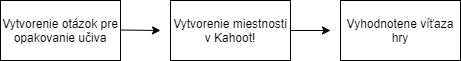
\includegraphics[width=10cm]{diagram.png}


\end{figure}

\subsection{Výhody aplikácie} \label{ina:este}
Každá aplikácia má svoje výhody. Aplikácia Kahoot! ich ma viacero a medzi najväčšie výhody aplikácie Kahoot! patrí: 
\begin{itemize}
\item	Učiteľ môže použiť Kahoot! presne pre ich špeciálne požiadavky. \cite{Lauren}. Ako som už spomínal v podkapitole vyššie, aplikácia Kahoot! je pre ovládanie veľmi jednoduchá a učiteľ si ju tak dokáže ľahko prispôsobovať podľa požiadaviek, ktorá si jeho hodina vyžaduje
\item	Deti zbožňujú túto aplikáciu najmä kvôli hravému prostrediu.\cite{Lauren} Aplikácia je totiž veľmi farebná a doslova lákavá najmä pre mladšie deti. 
\item	Super spôsob ako zapojiť technológie do učenia.\cite{Lauren}
\item	Kahoot! zapisuje aj nesprávne odpovede a študent si potom môže spätne pozrieť, že kde urobil chybu a poučiť sa do budúcna aby sa tejto chybe vyvarovali. \cite{Lauren}


\end {itemize}

\subsection{Nevýhody aplikácie}
Napriek viacerým výhodám prináša táto aplikácia aj určite nevýhody medzi, ktoré patria
\begin{itemize}
\item	Odpoveď môže byť iba krátka, v štýle áno, nie alebo viac správnych odpovedí, ale vývojári aplikácie sa to už snažia napraviť a snažia sa zlepšiť systém odpovedí. \cite{Lauren}
\item	Študenti získavajú bonusové body ak odpovedia čo najrýchlejšie a to môže spôsobiť, že niekedy sa študenti radšej ponáhľajú aby odpovedali čo najrýchlejšie, miesto toho aby sa zamysleli nad otázkou.\cite{Lauren}
\item	Študenti si síce môžu vymyslieť vlastné meno aby si zachovali anonymitu, ale aplikácia neumožňuje filtrovanie vulgárnych slov, preto sa v mene hráča môžu objaviť aj vulgarizmy \cite{nevyhoda}
\item	Študenti potrebujú na hranie hry mobil alebo iné zariadenie a zároveň pripojenie na internet. A práve pripojenie na internet nie je na väčšine škôl veľmi stabilné, čo môže spôsobovať výpadky počas hrania. \cite{nevyhoda}


\end {itemize}

\section{Experiment} \label{dolezita}
\textbf {Experiment z Univerzity technológii a vied v Nórsku.\cite{medina2017}} Účastníkmi tejto štúdie bolo 70 študentov angličtiny, ktorí študujú na Univerzite technológii a vied v Nórsku. Cieľom štúdie bolo ukázať ako pomáha aplikácia Kahoot! pri vyučovaní anglického jazyka. V štúdii môžeme vidieť porovnanie známok pred testom a porovnanie známok po teste. 
\begin{figure}[h] %obrázok
\centering
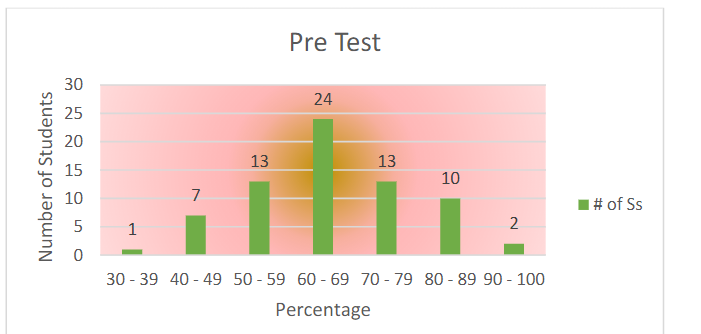
\includegraphics[width=9cm]{Predtestom.png}
\caption{
Výsledky pred testom\cite{medina2017}
}
\end{figure}

Na obrázku 2 môžeme vidieť graf výsledkov z testu študentov na hodinách anglického jazyka, predtým ako začali používať aplikáciu Kahoot!.Môžeme vidieť, že priemer dosahoval okolo 60 až 69 bodov. A až 8  z 30 študentov dosahovali výsledky menšie ako 50\%.
\begin{figure}[h] %obrázok
\centering
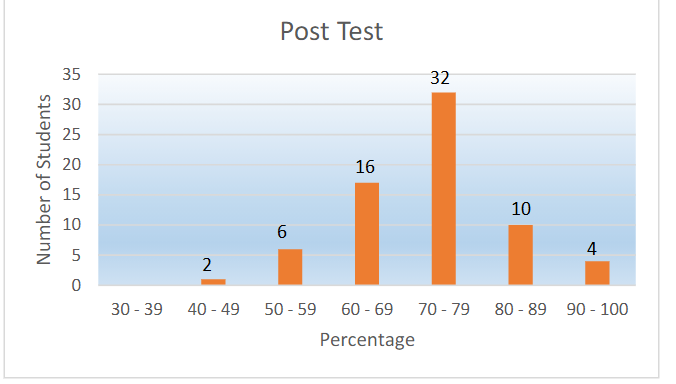
\includegraphics[width=9cm]{Poteste.png}
\caption{
Výsledky po teste\cite{medina2017}
}
\end{figure}

Na obrázku 3 môžeme vidieť graf výsledkov testu študentov na hodinách anglického jazyka po tom, čo začali používať aplikáciu Kahoot!. Môžeme vidieť, že priemer sa zvýšil a u každého študenta, môžeme zaznamenať progres. Priemer výsledkov sa zlepšil na 70 až 79 bodov. Celkovo môžeme vidieť, že táto aplikácia mala kladný dopad na študentov.

V závere štúdie bolo študentom položených zopár otázok aby zodpovedali ako sa im pracovalo v aplikácii a či im pomohla počas štúdia. Štatistika s výsledkami dotazníka je uvedená v tabuľke nižšie.

\begin{table}[tbh]
\centering
\begin{tabular}{@{}|l|c|c|c|@{}}
\toprule
Tvrdenie & Súhlasím(\%)  & Neviem(\%)  & Nesúhlasím(\%)  \\ \midrule
 1. Aplikácia Kahoot! je ľahká na použitie. & 100 & 0 & 0          \\ \midrule
 2. Vďaka Kahoot! som sa sústredil na úlohy. & 84 & 16 & 0        \\ \midrule
3. Radšej by som používal technológiu cez výučbu. & 83 & 9 & 8  \\ \midrule
4. Kahoot! má rozptyľoval. & 10 & 0 & 90\\ \midrule
5. Užíval som si použivanie aplikácie. & 95 & 5 & 0 
    \\ \midrule
6. Kahoot! ma pripravil na skúšky. & 74 & 18 & 8        \\ \bottomrule
\end{tabular}
\caption{\label{tab:Štatistika}Dotazník vyplnený študentami po teste}
\end{table}

Ako môžeme vidieť väčšina študentov si aplikáciu Kahoot! veľmi vychvaľovala najmä preto, že bola veľmi ľahká na používanie a zároveň sa vďaka nej  vedeli lepšie sústrediť na úlohy a to im pomohlo pri záverečnej skúške.
\bigskip

\section*{Záver} \label{zaver} 

Kahoot! a celkovo game-based learning sa v poslednej dobe stávajú súčasťou výučby najmä pre mladých žiakov. Stávajú sa súčasťou našej výučby kvôli tomu, lebo najmä pre malé deti je táto forma učenia viac zábavná a dokážu sa ľahšie naučiť a zapamätať si nové veci.

V prvej sekcii sme si zadefinovali pojem game-based learning, ktorého aplikácia Kahoot! je súčasťou. V druhej sekcii sme sa venovali samotnej aplikácii Kahoot! ako vyzerá a v pod sekciách sme sa venovali tomu, ako prebieha výučba pomocou tejto aplikácie ale aj jej výhodám a nevýhodám. V tretej sekcii sme sa pozreli na experiment v Nórsku, kde sme mohli vidieť výrazne zlepšenie študentov vďaka tejto aplikácii

Hlavný cieľ tejto práce, ktorým bolo povedať čo je to game-based learning a najmä opísať aplikáciu Kahoot!, ktorá sa v tomto smere používa momentálne najčastejšie sa nám podarilo splniť. Uviedli sme si všetko, čo sa ku tejto aplikácii dalo a zistili sme, že táto aplikácia má pozitívny dopad na študentov pri učení. 



\section*{Reakcia na prednášky}
\paragraph{Spoločenské súvislosti.}
Ohľadom dopadu na spoločnosť by sme mohli spomenúť, že spoločnosť sa čoraz viac a viac digitalizuje a môžeme vidieť, že sa to prenáša už aj do škôl. To môžeme síce hodnotiť ako pozitívum, ale ešte nie každý v dnešnej dobe má mobilné zariadenie. Mobilné zariadenie v súčastnosti vlastní 44,81\% ľudskej populácie\cite{Turner2020}, to znamená, že je ešte veľa študentov, ktorí si nemôžu dovoliť alebo z iných príčin nemajú zariadenie na používanie aplikácie Kahoot!. 
\paragraph{Historické súvislosti.}
Ku histórii toho môžeme spomenúť zatiaľ len veľmi málo. História ohľadom zapájania technológii do štúdia je totižto ešte v plienkach, keďže hry ako súčasť učenia sa začali implementovať do škôl len nedávno. Vďaka silnému rozvoju IT, ale môžeme očakávať, že tento trend sa bude naďalej rozvíjať. 
\paragraph{Technológia a ľudia.}
Vývoj nových technológii a najmä vývoj moderných mobilov umožnil študentom uľahčenie viacerých foriem učenia. V dnešnej dobe si totižto všetky potrebné informácie ku škole môžeme pohľadať na internete. Pozitívny fakt ale je ten, že škola nezanevrela na tieto objavy ale práve naopak sa ich  snaží použiť ako formu učenia, čo môžeme sledovať práve pri tejto aplikácii a vďaka tomu sa modernej mládeži zlepšujú výsledky.  
\paragraph{Udržateľnosť a etika.}
Udržateľnosť tejto aplikácie na škole a celkovo aj táto metóda učenia je vysoko pravdepodobná. Táto aplikácia totiž dosahuje vysoké percento úspešnosti a viacero študentov si ju pochvaľuje, že im umožnila lepšie pochopiť nové učivo. Netreba ale zabúdať, že aj napriek tomu treba dodržiavať nejakú etiku aj pri používaní tejto aplikácie. Nedávať si vulgárne meno pri používaní tejto aplikácie, alebo sa nevysmievať tým čo prehrali. 

%\acknowledgement{Ak niekomu chcete poďakovať\ldots}



\bibliography{literatura}
\bibliographystyle{plain} % prípadne alpha, abbrv alebo hociktorý iný
\end{document}